\documentclass[11pt,a4paper]{article}

% ── Compilar con: tectonic x5_alt_v2_opus.tex  (motor XeTeX, UTF-8 nativo) ──
\usepackage{fontspec}
\usepackage{amsmath,amssymb}
\usepackage[margin=2.3cm]{geometry}
\usepackage{xcolor}
\usepackage{booktabs}
\usepackage{tabularx}
\usepackage{enumitem}
\usepackage{underscore}
\usepackage{titlesec}
\usepackage{caption}
\usepackage{pgfplots}
\pgfplotsset{compat=1.18}
\usepackage[hidelinks]{hyperref}

% ── Colores (mismos que docs/plans/x5_alt_v2.tex) ──
\definecolor{cazul}{HTML}{2C5F8A}
\definecolor{cverde}{HTML}{2E8B57}
\definecolor{cnaranja}{HTML}{C1660A}
\definecolor{cmorado}{HTML}{6B4FA0}
\definecolor{cgris}{HTML}{5B6770}
\definecolor{crojo}{HTML}{B3261E}
% Series de gráficos (paleta categórica validada: azul, naranja)
\definecolor{serieA}{HTML}{2A78D6}
\definecolor{serieB}{HTML}{EB6834}
\definecolor{tinta2}{HTML}{52514E}

\setlist{itemsep=2pt, topsep=4pt}
\emergencystretch=3em
\captionsetup{font=small, labelfont=bf, labelsep=period}
\renewcommand{\contentsname}{Índice}
\renewcommand{\tablename}{Tabla}
\renewcommand{\figurename}{Figura}
\titleformat{\section}{\normalfont\Large\bfseries\color{cazul}}{\thesection}{0.6em}{}
\titleformat{\subsection}{\normalfont\large\bfseries\color{cazul}}{\thesubsection}{0.6em}{}
\titlespacing*{\section}{0pt}{2.2ex plus 1ex minus .2ex}{1.0ex plus .2ex}
\titlespacing*{\subsection}{0pt}{1.8ex plus 1ex minus .2ex}{0.8ex plus .2ex}

\newcommand{\code}[1]{\texttt{\small #1}}

\newenvironment{caja}[1]{%
  \par\medskip\noindent
  \begin{tabular}{@{}p{0.4em}@{\hspace{8pt}}p{\dimexpr\linewidth-2em\relax}@{}}
  \textcolor{#1}{\rule{3pt}{1.1em}} &
}{\end{tabular}\par\medskip}
\newenvironment{nota}{\begin{caja}{cnaranja}}{\end{caja}}
\newenvironment{clave}{\begin{caja}{cmorado}}{\end{caja}}
\newenvironment{advertencia}{\begin{caja}{crojo}}{\end{caja}}

\pgfplotsset{
  estilo/.style={
    axis line style={tinta2!60}, tick style={tinta2!60},
    major grid style={gray!18}, tick label style={font=\footnotesize, color=black},
    label style={font=\footnotesize, color=tinta2},
    legend style={font=\footnotesize, draw=none, fill=none},
    legend cell align=left,
  },
}

\title{\vspace{-1.6cm}\textbf{{\ttfamily X5\_alt\_v2} — revisión crítica independiente}\\[6pt]
  \large Qué está bien, qué no se sostiene y qué haría a continuación\\[4pt]
  \normalsize\color{cgris} Revisión de la planificación, de \code{X5\_Q1}–\code{X5\_Q4} y del diseño de \code{X5\_Q5}}
\author{Claude (Opus 5.5) para Mauricio Valdivia}
\date{23 de octubre de 2026}

\begin{document}
\maketitle
\vspace{-0.6cm}

% ════════════════════════════════════════════════════════════════════
\section*{Resumen ejecutivo}

Me pediste revisar \code{X5\_alt\_v2} completo, cuestionarlo y decir si tiene potencial. Lo revisé
leyendo toda la documentación y los cuatro notebooks, y además corrí análisis propios sobre los
datos que ya exportaste a Mac (\code{exp\_Q1} y \code{exp\_Q4}, con velas hasta el 17-oct-2026).
Mi lectura, en corto:

\begin{enumerate}[leftmargin=1.4em]
  \item \textbf{La pregunta es buena y la disciplina de trabajo es excelente.} Separar investigación de
        producción, pre-registrar hipótesis, trabajar por activo, cuidar la causalidad y dejar cada
        decisión con su descarte es mucho más riguroso que lo habitual en un proyecto personal. El
        diseño de \code{Q5} (control estático pareado, sorteo aleatorio, tramo final intocable y
        compuerta manual) es lo mejor del plan.
  \item \textbf{Pero hasta hoy \code{X5\_alt\_v2} no ha producido evidencia empírica sobre ningún parámetro.}
        La evidencia ``alta'' de \code{Q3} para \code{N} y \code{K} es mecánica: correlaciona cada
        variable con el retorno \emph{de la misma vela}, que la variable ya contiene. Con el retorno de
        la vela siguiente, la correlación cae a cero (Sección~\ref{sec:mecanica}).
  \item \textbf{La calibración de \code{Q4} no puede fallar.} Su objetivo es el percentil del propio
        índice, así que el ajuste sale bien con cualquier variable: el indicador de fuerza relativa
        (RSI) da $R^2=0.98$ y el ruido puro $0.998$. Invertir la hipótesis de \code{N} da exactamente el
        mismo $R^2$ y el mismo signo ``correcto'' (Sección~\ref{sec:q4}). \code{Q4} aporta una
        \emph{parametrización}, no una calibración.
  \item \textbf{El \code{N} dinámico actual es, ante todo, un \code{N} más bajo}: promedia 117--135
        soportes contra 180 fijos y está bajo el valor estático el 95--100\% del tiempo. Si \code{Q5}
        lo compara contra el estático, va a medir nivel y no dinamismo (Sección~\ref{sec:nivel}).
  \item \textbf{El mecanismo económico de \code{N} es de riesgo, no de retorno.} En los estados
        adversos el retorno de los 7 días siguientes no es peor en promedio, pero la caída máxima
        posterior es $\sim$50\% mayor. Con la métrica decidida para \code{Q5} (retorno total) la
        hipótesis se evaluaría con la vara equivocada (Sección~\ref{sec:riesgo}).
  \item \textbf{Hay problemas de unidades que conviene resolver antes que cualquier dinamismo}: las
        ventanas están en barras (para acciones, ``30 días'' son 72 a 103 días de mercado) y \code{A},
        \code{B} y \code{PERDIDA\_MAX} están en dólares, de modo que el valor ``estático'' de hoy ya
        cambia muchísimo en términos de mercado entre activos y entre años (Secciones~\ref{sec:ventanas}
        y~\ref{sec:unidades}).
  \item \textbf{La configuración actual gana poco y seguido, y pierde mucho y rara vez}: en BTCUSD la
        ganancia mínima asegurada es 3 USD por posición y la pérdida máxima 400 USD; en GOOGL, NVDA y AMZN
        la pérdida máxima ni siquiera se habría activado en 2022--2026. Por eso \code{Q5} tiene que medir
        el valor de mercado de la cuenta (cerrado más flotante), no el dinero cerrado
        (Sección~\ref{sec:asimetria}).
\end{enumerate}

\begin{clave}
\textbf{¿Tiene potencial?} Sí, pero no donde el plan lo está buscando. El valor más probable está en
(a) \emph{normalizar} \code{A}/\code{B}/\code{PERDIDA\_MAX} por volatilidad, que ya cumple la
hipótesis ``volatilidad alta $\rightarrow$ A alto'' sin ningún modelo; (b) usar \code{N} como
\emph{freno de riesgo} evaluado con métricas ajustadas por riesgo; y (c) el arnés experimental de
\code{Q5}, que sirve para probar cualquier cambio futuro de X0/X1. Mi recomendación central: no
seguir \code{Q4} parámetro por parámetro con tres compuertas cada uno; cerrarlo como parametrización
y pasar cuanto antes a un piloto chico y decisivo de \code{Q5} (Sección~\ref{sec:plan}).
\end{clave}

% ════════════════════════════════════════════════════════════════════
\section{Qué revisé y cómo}

\textbf{Documentos}: \code{x5\_contexto\_conversacion.md} (documento rector), \code{plan\_x5\_alt\_v2.md},
\code{X5\_alternativo.md} (§10), \code{pars\_configurables.md}, \code{estandar\_reportes\_investigacion.md},
las entradas de \code{decisiones.md} desde el 17-oct, la sección \code{X5\_alt\_v2} de \code{todos.md} y
\code{done.md}, y las últimas minutas de \code{records.md}. \textbf{Código}: los cuatro notebooks
\code{X5\_Q1}–\code{X5\_Q4} (celdas y salidas), \code{x5\_alt\_funciones.py}, \code{x5\_alt\_export.py},
\code{config.py} y las partes de \code{X0}/\code{X1} que tocan \code{N}, \code{A}, \code{B}, \code{K} y
\code{N\_EXP}.

\textbf{Análisis propios} (detalle en el Anexo): correlaciones contemporáneas contra futuras, ajuste de
\code{Q4} sobre variables sin contenido económico, distribución y rotación de $\hat N$, resultado
futuro del precio por estado del activo, escala de \code{A}/\code{B}/\code{PERDIDA\_MAX} en unidades
de mercado, estabilidad de la calibración y densidad real de los soportes de producción.

\begin{nota}
\textbf{Qué no hice}: no corrí backtesting (requiere Windows/MT5 y la interfaz de \code{Q5-1}) y no
modifiqué ningún notebook ni el plan. Todo lo de este documento son hallazgos y propuestas; las
decisiones son tuyas. Los números son descriptivos: ventanas solapadas, un solo período (2022--2026)
y sin pruebas de significancia formales.
\end{nota}

% ════════════════════════════════════════════════════════════════════
\section{Lo que está bien (y conviene conservar)}

\begin{itemize}[leftmargin=1.2em]
  \item \textbf{Investigación separada de producción.} Nada de \code{Q1}–\code{Q5} toca X0/X1 y el
        traspaso futuro tiene compuerta manual. Con dinero real, es exactamente lo correcto.
  \item \textbf{Documento rector y pre-registro de hipótesis} (\code{PRE-1}) antes de correr nada.
        Escribir la dirección esperada antes de ver datos es la mejor defensa contra encontrar lo que
        uno quiere ver.
  \item \textbf{Análisis por activo y sin variables de cuenta.} Evita mezclar el estado del mercado
        con el estado de tu cartera, que es la confusión más común en este tipo de sistemas.
  \item \textbf{Cuidado con la causalidad}: el percentil causal y el promedio móvil exponencial (EMA)
        causal no usan información futura, y está documentado por qué.
  \item \textbf{Trazabilidad}: cada decisión tiene motivo y alternativa descartada. Gracias a eso esta
        revisión fue posible en una sesión.
  \item \textbf{Honestidad intelectual}: el propio notebook \code{Q4} ya dice que el $R^2$ sale alto
        ``casi por construcción''. Este documento lleva esa intuición hasta sus consecuencias.
  \item \textbf{El diseño de \code{Q5}}: control estático pareado por ventana (cancela el efecto del
        mercado de esa semana), coeficientes sorteados (evita sesgo de selección), evaluación solo en la
        cola nueva y un tramo final que nadie mira. Es un diseño experimental serio.
\end{itemize}

% ════════════════════════════════════════════════════════════════════
\section{Hallazgos}

Cada hallazgo sigue el mismo orden: qué encontré, por qué importa y qué propongo. Están ordenados por
impacto sobre las decisiones que vienen.

% ────────────────────────────────────────────────────────────────────
\subsection{La evidencia ``alta'' de Q3 para N y K es mecánica}\label{sec:mecanica}

\textbf{Qué encontré.} \code{Q2} mide cada variable contra \code{retorno\_log\_1h}, que es
$\ln(C_t/C_{t-1})$: el retorno de la \emph{misma} vela en que se calcula la variable. \code{Q3}
interpreta esa correlación como relación ``con el retorno siguiente'', pero no lo es. Y para las
variables de drawdown y de ruptura de rango la correlación es casi obligatoria: si la última hora subió
1\%, el cierre se acerca a su máximo reciente (el drawdown sube hacia 0) y es más probable que supere el
máximo de las 20 velas previas (la ruptura marca $+1$). La variable \emph{contiene} el retorno que se
le está correlacionando.

Lo comprobé con los datos de los 7 activos: basta con desplazar el retorno una vela hacia adelante para
que la correlación desaparezca (Figura~\ref{fig:mecanica}). Lo mismo ocurre con el retorno de las 24
horas o los 7 días siguientes (todas las correlaciones quedan entre $-0.05$ y $+0.03$).

\begin{figure}[h]
\centering
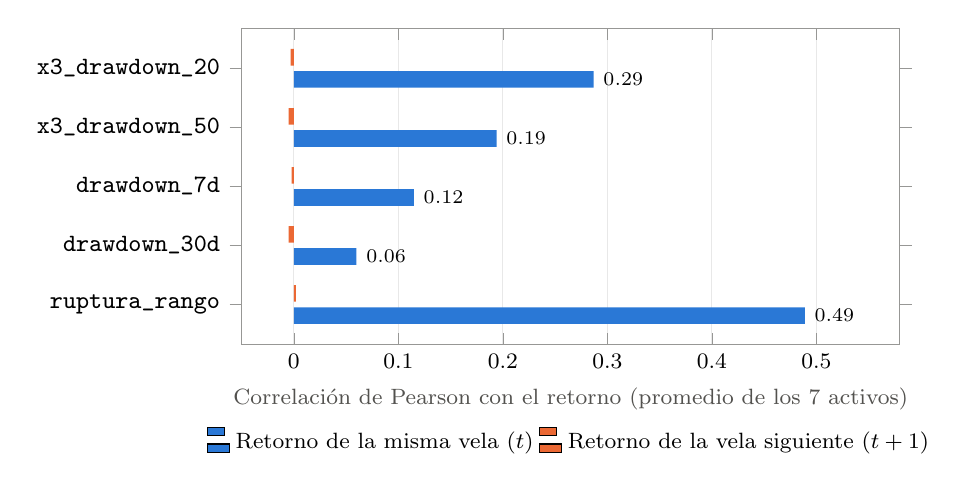
\begin{tikzpicture}
\begin{axis}[estilo, xbar, width=0.82\linewidth, height=5.6cm,
  y dir=reverse, ytick={1,2,3,4,5}, enlarge y limits=0.17, bar width=6pt,
  yticklabels={\code{x3\_drawdown\_20}, \code{x3\_drawdown\_50}, \code{drawdown\_7d}, \code{drawdown\_30d}, \code{ruptura\_rango}},
  xmin=-0.05, xmax=0.58, xtick={0,0.1,0.2,0.3,0.4,0.5}, scaled x ticks=false,
  xticklabel style={/pgf/number format/fixed, /pgf/number format/precision=1}, xmajorgrids,
  xlabel={Correlación de Pearson con el retorno (promedio de los 7 activos)},
  legend style={at={(0.5,-0.24)}, anchor=north}, legend columns=2]
\addplot[fill=serieA, draw=none, nodes near coords, every node near coord/.append style={font=\scriptsize, color=black},
  nodes near coords={\pgfmathprintnumber[fixed, zerofill, precision=2]{\pgfplotspointmeta}}, point meta=x]
  coordinates {(0.287,1) (0.194,2) (0.115,3) (0.060,4) (0.489,5)};
\addplot[fill=serieB, draw=none] coordinates {(-0.003,1) (-0.005,2) (-0.002,3) (-0.005,4) (0.002,5)};
\legend{Retorno de la misma vela ($t$)\quad, Retorno de la vela siguiente ($t+1$)}
\end{axis}
\end{tikzpicture}
\caption{La correlación que \code{Q3} clasificó como evidencia ``alta'' (barras azules) desaparece al
mirar el retorno siguiente (barras naranjas). En BTCUSD: \code{x3\_drawdown\_20} pasa de $0.278$ a
$-0.010$ y \code{ruptura\_rango} de $0.500$ a $-0.003$.}
\label{fig:mecanica}
\end{figure}

\textbf{Por qué importa.} La tabla final de \code{Q3} marca \code{N} con prioridad ``alta'' porque sus
variables tenían ``evidencia Q2-11 alta y estable''; esa justificación no existe. Para \code{A},
\code{factor\_B} y \code{N\_EXP} la evidencia ``baja'' tampoco dice nada, porque el retorno de una vela
no es el resultado que esos parámetros afectan (el documento rector ya lo advierte en §17). En
consecuencia, hoy las hipótesis de los siete parámetros descansan solo en intuición de dominio. Eso es
legítimo, pero hay que decirlo así para no tomar decisiones creyendo que hay datos detrás.

\textbf{Qué propongo.} Corregir el registro en \code{X5\_alternativo.md} §10.5 y en
\code{plan\_x5\_alt\_v2.md} §2 (una nota basta) y dejar de usar \code{nivel\_evidencia\_q2} como criterio
de prioridad. La única evidencia que importa para un parámetro es el resultado de operar con él, y esa
llega recién en \code{Q5}.

% ────────────────────────────────────────────────────────────────────
\subsection{La calibración de Q4 no puede fallar}\label{sec:q4}

\textbf{Qué encontré.} En \code{Q4}, el objetivo $y^*_t$ es el percentil causal del propio índice
$s_t$, reescalado al rango del parámetro. La sigmoide termina aproximando la distribución acumulada de
$s_t$, que es una curva creciente en forma de S para \emph{cualquier} variable. Lo probé pasando por
\code{calibrar\_parametro} (sin modificarlo) variables que no tienen nada que ver con la hipótesis
(Figura~\ref{fig:r2}).

\begin{figure}[h]
\centering
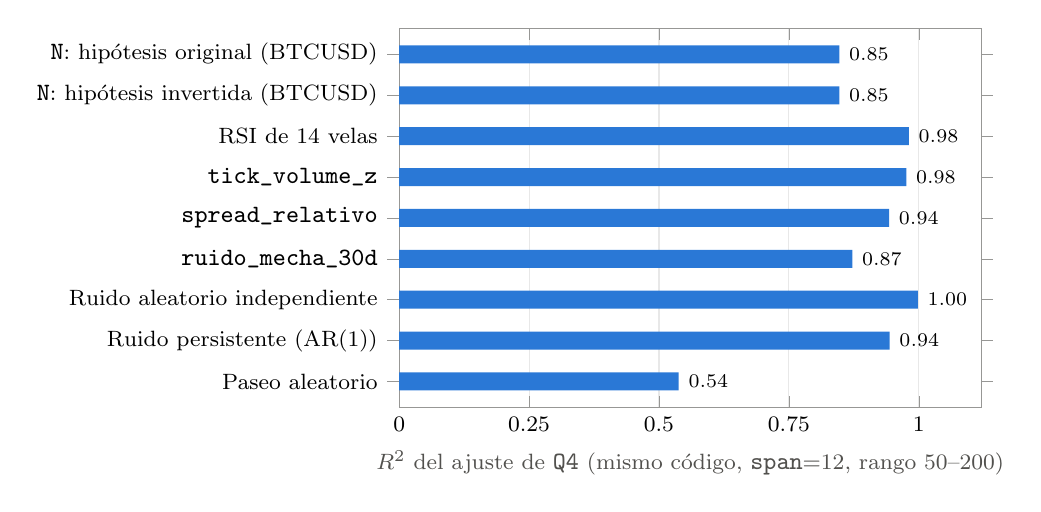
\begin{tikzpicture}
\begin{axis}[estilo, xbar, width=0.74\linewidth, height=6.4cm,
  y dir=reverse, ytick={1,...,9}, enlarge y limits=0.08, bar width=6.5pt,
  yticklabels={\code{N}: hipótesis original (BTCUSD), \code{N}: hipótesis invertida (BTCUSD), RSI de 14 velas, \code{tick\_volume\_z}, \code{spread\_relativo}, \code{ruido\_mecha\_30d}, Ruido aleatorio independiente, Ruido persistente (AR(1)), Paseo aleatorio},
  xmin=0, xmax=1.12, xtick={0,0.25,0.5,0.75,1}, xmajorgrids,
  xlabel={$R^2$ del ajuste de \code{Q4} (mismo código, \code{span}=12, rango 50--200)},
  nodes near coords, every node near coord/.append style={font=\scriptsize, color=black},
  nodes near coords={\pgfmathprintnumber[fixed, zerofill, precision=2]{\pgfplotspointmeta}}, point meta=x]
\addplot[fill=serieA, draw=none] coordinates {(0.847,1) (0.847,2) (0.981,3) (0.976,4) (0.943,5) (0.872,6) (0.998,7) (0.944,8) (0.538,9)};
\end{axis}
\end{tikzpicture}
\caption{$R^2$ de la calibración de \code{Q4}. Variables reales sin relación con la hipótesis y series
sintéticas sin ningún contenido económico ajustan tan bien o mejor que el índice de \code{N}. El único
caso bajo es el paseo aleatorio, por no ser estacionario.}
\label{fig:r2}
\end{figure}

Tres consecuencias directas:
\begin{itemize}[leftmargin=1.2em]
  \item \textbf{El chequeo de signo no puede fallar.} Como el percentil crece con $s$, la pendiente
        ajustada es siempre positiva. Invertir la hipótesis de \code{N} (drawdown profundo y volatilidad
        alta $\rightarrow$ \code{N} \emph{alto}) da $R^2=0.847$ y pendiente $1.891$, idénticos al original.
        La dirección la pone quien elige el signo de cada variable, no los datos.
  \item \textbf{\code{punto\_medio} y \code{pendiente} describen la forma de $s_t$, no la economía.}
        La pendiente ajustada queda entre 0.67 y 0.96 veces la de una curva normal con la misma
        desviación de $s_t$ en los 7 activos; el punto medio queda algo bajo la mediana de $s_t$ porque
        el percentil es acumulado desde 2022.
  \item \textbf{El $R^2$ no sirve para elegir nada.} Ya lo detectaste al sacar \code{w\_1} de la grilla
        por $R^2$. Aplica igual a elegir variables, ventanas o \code{span}.
\end{itemize}

\textbf{Por qué importa.} Lo que \code{Q4} realmente decide son cinco elecciones humanas: qué
variables, con qué signo, entre qué piso y techo, con cuánto suavizado y con qué pesos. Eso es una
\emph{parametrización}, y es útil, pero no justifica tres compuertas secuenciales (implementar, ejecutar
en Windows, revisar visuales) por cada uno de los seis parámetros que faltan: son unas 20 iteraciones
con muy poca información por iteración.

\textbf{Qué propongo.} Declarar \code{Q4} como ``parametrización'' y cerrar \code{N} tal como está. Para
el resto, ver la Sección~\ref{sec:plan}: algunos parámetros no necesitan sigmoide y otros no deberían
ser dinámicos. Los coeficientes de la curva pasan a ser dimensiones de búsqueda de \code{Q5}, que es lo
que \code{Q5-1} ya contempla.

% ────────────────────────────────────────────────────────────────────
\subsection{El N dinámico es, sobre todo, un N más bajo}\label{sec:nivel}

\textbf{Qué encontré.} Por construcción, el percentil reparte el tiempo de forma pareja entre piso y
techo, así que $\hat N$ vive en promedio cerca del centro del rango. El valor estático, en cambio,
está en el borde: 180, que para las acciones \emph{es} el techo. Resultado: el \code{N} dinámico está
bajo el estático casi siempre (Tabla~\ref{tab:nivel}).

\begin{table}[h]
\centering\small
\begin{tabular}{lcccccc}
\toprule
Activo & Rango & Media $\hat N$ & Mediana & p10--p90 & \% tiempo bajo 180 & Cambios/día (paso 10) \\
\midrule
BTCUSD & 50--200 & 135 & 148 & 69--177 & 95\% & 1.5 \\
ETHUSD & 50--200 & 129 & 140 & 65--172 & 99\% & 1.4 \\
TSLA   & 40--180 & 121 & 134 & 58--162 & 100\% & 0.7 \\
GOOGL  & 40--180 & 117 & 122 & 63--157 & 100\% & 0.4 \\
NVDA   & 40--180 & 124 & 135 & 67--156 & 100\% & 0.5 \\
AMZN   & 40--180 & 119 & 130 & 60--151 & 100\% & 0.5 \\
MSFT   & 40--180 & 118 & 127 & 59--162 & 100\% & 0.6 \\
\bottomrule
\end{tabular}
\caption{Distribución de $\hat N$ (export de \code{Q4} con \code{drawdown\_30d}, $w_1=0.7$, \code{span}=12).
La última columna cuenta cuántas veces por día con datos cambia $\hat N$ redondeado a múltiplos de 10.}
\label{tab:nivel}
\end{table}

\textbf{Por qué importa.} Si \code{Q5} encuentra que el dinámico rinde 3\% más que el estático, no
sabremos si fue por \emph{cuándo} baja \code{N} o simplemente porque operó con 50 soportes menos en
promedio. Un \code{N} fijo de 125 podría lograr lo mismo sin ninguna maquinaria.

\textbf{Qué propongo.} Agregar a \code{Q5} un control estático \emph{igualado}: \code{N} fijo igual al
promedio de $\hat N$ del mismo período. La pregunta ``¿sirve el dinamismo?'' se responde con dinámico
contra estático igualado; la pregunta ``¿180 es buen nivel?'' con estáticos de distinto nivel entre sí.
Alternativa equivalente: centrar el rango en el valor estático (por ejemplo, 120--240) para que ambos
operen con el mismo \code{N} medio.

% ────────────────────────────────────────────────────────────────────
\subsection{El mecanismo económico de N es de riesgo, no de retorno}\label{sec:riesgo}

\textbf{Qué encontré.} Antes de gastar en backtesting se puede mirar algo barato: qué hizo el precio
\emph{después} de cada estado. Dividí las velas de cada activo en cinco grupos según $s_t$ (el índice de
\code{N}) y medí el retorno de los 7 días siguientes y la caída máxima dentro de esos 7 días, también
llamada excursión adversa máxima (MAE, \emph{Maximum Adverse Excursion}).

\begin{figure}[h]
\centering
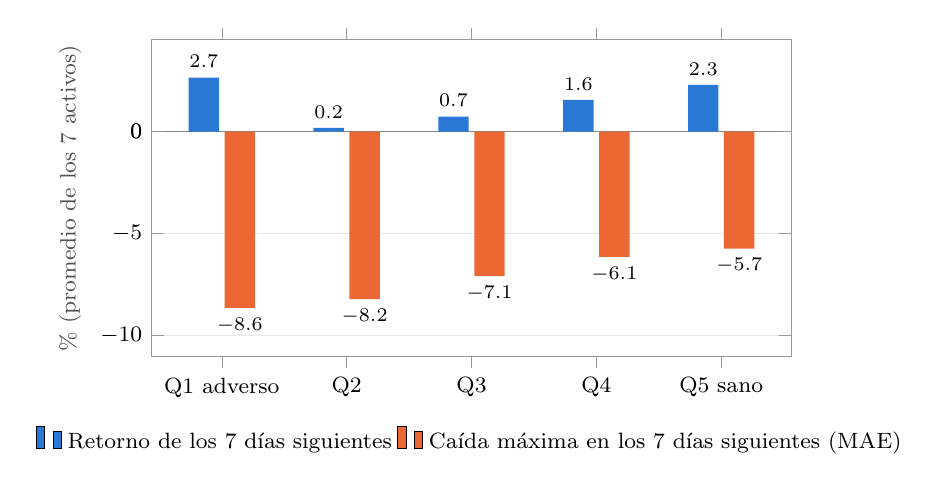
\begin{tikzpicture}
\begin{axis}[estilo, ybar, width=0.8\linewidth, height=5.6cm, bar width=11pt,
  symbolic x coords={q1,q2,q3,q4,q5}, xtick=data,
  xticklabels={Q1 adverso, Q2, Q3, Q4, Q5 sano},
  ymin=-11, ymax=4.5, ymajorgrids, ylabel={\% (promedio de los 7 activos)},
  extra y ticks={0}, extra y tick style={grid=major, major grid style={tinta2!70}},
  legend style={at={(0.5,-0.2)}, anchor=north}, legend columns=2, enlarge x limits=0.14,
  nodes near coords, every node near coord/.append style={font=\scriptsize, color=black},
  nodes near coords={\pgfmathprintnumber[fixed, precision=1]{\pgfplotspointmeta}}]
\addplot[fill=serieA, draw=none] coordinates {(q1,2.65) (q2,0.18) (q3,0.73) (q4,1.56) (q5,2.29)};
\addplot[fill=serieB, draw=none] coordinates {(q1,-8.64) (q2,-8.21) (q3,-7.08) (q4,-6.14) (q5,-5.73)};
\legend{Retorno de los 7 días siguientes\quad, Caída máxima en los 7 días siguientes (MAE)}
\end{axis}
\end{tikzpicture}
\caption{Resultado futuro del precio según el estado del activo medido por el índice de \code{N}. El
retorno posterior no empeora en los estados adversos; la caída posterior sí es mayor en todos los activos.}
\label{fig:riesgo}
\end{figure}

El patrón de la caída máxima se repite en los 7 activos sin excepción (estado adverso contra sano: BTC
$-6.2\%$ vs $-4.2\%$, ETH $-9.0\%$ vs $-5.9\%$, NVDA $-10.7\%$ vs $-5.0\%$). El del retorno no: en
cripto, el retorno a 30 días sí es peor en estado adverso (BTC $-0.5\%$ vs $+3.7\%$; ETH $-0.1\%$ vs
$+2.9\%$), mientras que en varias acciones es mejor (TSLA $+14.4\%$ vs $-6.1\%$; AMZN y MSFT también
rebotan).

\textbf{Por qué importa.} Alginvesting compra caídas en soportes. Bajar \code{N} en estado adverso
significa comprar menos justo cuando el precio cae más (menor riesgo) pero también cuando, en acciones,
suele rebotar (menor retorno). La hipótesis de \code{N} es, en el fondo, una regla de \emph{gestión de
riesgo}. La decisión del 23-oct fija como métrica de \code{Q5} el retorno total, reportando el drawdown
sin optimizarlo. Con esa vara, una regla que reduce el riesgo a la mitad perdiendo un poco de retorno
se descartaría, y una que solo baja el nivel medio de \code{N} podría ganar por accidente.

\textbf{Qué propongo.} (1) Que el objetivo de \code{Q5} sea ajustado por riesgo: retorno dividido por
drawdown máximo, o retorno con un tope de drawdown como restricción. (2) Reportar también el retorno por
unidad de capital comprometido, porque con menos \code{N} hay menos capital expuesto y comparar retorno
bruto castiga eso injustamente. (3) La diferencia cripto/acciones respalda tu decisión de probar la
agregación por \code{tipo\_valor} (\code{Q5-3}). La literatura apunta en la misma dirección: reducir
exposición cuando sube la volatilidad mejora el resultado ajustado por riesgo en muchas estrategias
(Moreira y Muir, 2017, \emph{Volatility-Managed Portfolios}), no necesariamente el bruto.

% ────────────────────────────────────────────────────────────────────
\subsection{Las ventanas están en barras, no en tiempo}\label{sec:ventanas}

\textbf{Qué encontré.} Todas las ventanas de \code{Q1}/\code{X3} se definen en número de velas
suponiendo 24 velas por día. En cripto es cierto; en acciones no (Tabla~\ref{tab:ventanas}).

\begin{table}[h]
\centering\small
\begin{tabular}{lcccc}
\toprule
Activo & Velas/día & ``30d'' (720 velas) & ``7d'' (168 velas) & EMA \code{span}=12 \\
\midrule
BTCUSD, ETHUSD & 24 & 30 días & 7 días & 12 horas \\
TSLA, NVDA, AMZN, MSFT & 10 & 72 días de mercado & 17 días & 1.2 días \\
GOOGL & 7 & 103 días de mercado & 24 días & 1.7 días \\
\bottomrule
\end{tabular}
\caption{Horizonte real de cada ventana según el activo (velas por día con datos, 2022--2026).}
\label{tab:ventanas}
\end{table}

\textbf{Por qué importa.} Las comparaciones del 23-oct entre \code{drawdown\_7d}, \code{30d} y \code{60d}
se hicieron sobre los 7 activos como si fueran el mismo horizonte; para acciones, ``30d'' ya es más de
tres meses. Lo mismo con \code{cambio\_volatilidad} (24/168 velas), con el EMA y con la anualización
$\sqrt{8760}$, que en acciones no corresponde (esta última solo afecta la escala). Además, GOOGL tiene
7 velas por día y las otras acciones 10: su sesión en el bróker es distinta, por eso tiene menos filas.
No descartaría que la anomalía de TSLA (\code{falso\_sano} alto con cualquier ventana) tenga que ver con
esto.

\textbf{Qué propongo.} Definir las ventanas en tiempo calendario (\code{rolling('30D')} sobre un índice de
fechas) o en días de mercado por tipo de activo, y expresar \code{span} en horas o días. Es un cambio
chico en \code{Q1} y evita que cada conclusión entre activos quede contaminada.

% ────────────────────────────────────────────────────────────────────
\subsection{\texorpdfstring{A, B y \code{PERDIDA\_MAX}}{A, B y PERDIDA_MAX} están en dólares; el mercado no}\label{sec:unidades}

\textbf{Qué encontré.} X1 escala \code{A}, \code{B} y \code{PERDIDA\_MAX} por el lote real de cada
posición, así que los tres equivalen a una \emph{distancia de precio} fija: el monto en USD dividido por
$L_{\min} = \code{MIN\_LOTAJES}\cdot\code{UNITS}$. Por ejemplo, en BTCUSD \code{A}=3 USD exige 300 USD de
distancia en precio, tanto para crear una Orden en Espera (OE) como para activar el primer stop ganador.
Medida en unidades de volatilidad, el promedio del rango verdadero de una vela (ATR, \emph{Average True
Range}), esa distancia es muy distinta entre activos (Tabla~\ref{tab:unidades}) y también cambia mucho en
el tiempo: en BTCUSD pedía 1.9 ATR en 2023 y 0.5 ATR en 2025; en NVDA, 11.4 ATR en 2022 y 1.7 ATR en
2026, porque el precio subió diez veces y los 3 USD quedaron iguales.

\begin{table}[h]
\centering\small
\begin{tabular}{lrcccc}
\toprule
Activo & Precio mediano & \code{A} & \code{B} & \code{PERDIDA\_MAX} & ¿\code{PERDIDA\_MAX} se habría \\
       & (últimos 365 d) & (en ATR) & (en ATR) & (\% del precio) & activado en 2022--2026? \\
\midrule
BTCUSD & 77\,303 & 0.64 & 0.32 & 25.9\% & Sí \\
ETHUSD & 2\,320 & 1.59 & 0.79 & 86.2\% & Sí \\
TSLA   & 399 & 0.73 & 0.37 & 50.1\% & Sí \\
GOOGL  & 335 & 1.14 & 0.57 & 59.6\% & No \\
NVDA   & 197 & 1.69 & 0.85 & 101.5\% & No \\
AMZN   & 243 & 1.69 & 0.85 & 82.5\% & No \\
MSFT   & 448 & 0.99 & 0.50 & 44.6\% & Sí (por poco) \\
\bottomrule
\end{tabular}
\caption{Los valores ``estáticos'' de \code{config.py} expresados como distancia de precio, en ATR de
velas H1 y en porcentaje del precio. La última columna indica si la mayor caída observada desde un cierre
hasta un mínimo posterior supera la distancia de \code{PERDIDA\_MAX}, es decir, si se habría activado
incluso comprando en el peor momento.}
\label{tab:unidades}
\end{table}

\textbf{Por qué importa.} Tres cosas. (1) El ``estático'' contra el que \code{Q5} va a comparar ya es,
en la práctica, un parámetro que se mueve con el precio, y en sentido contrario al que sugiere la
hipótesis. (2) El plan de \code{Q4} para \code{A} (sigmoide sobre el percentil de \code{x3\_atr\_pct}
llevada a un rango fijo de 2--20 USD) conserva el problema: el percentil olvida el nivel de precio, así
que el mismo percentil de volatilidad daría los mismos dólares con BTC a 20\,000 o a 120\,000.
(3) \code{PERDIDA\_MAX} equivale a caídas de 26\% a 102\% del precio: en GOOGL, NVDA y AMZN no se habría
activado nunca en todo el período. En la práctica, esas posiciones operan sin stop de pérdida.

\textbf{Qué propongo.} Antes de cualquier dinamismo, expresar \code{A} como un múltiplo de la
volatilidad: $A_t = k_A \cdot \mathrm{ATR}_t \cdot L_{\min}$, y lo mismo para $B_t = k_B \cdot
\mathrm{ATR}_t \cdot L_{\min}$ (con lo que $\text{factor\_B} = k_B/k_A$). Eso \emph{ya es} la hipótesis
``volatilidad alta $\rightarrow$ \code{A} alto'', con un solo número por parámetro, sin sigmoide, sin
percentil y con sentido físico claro (``exigir 1 ATR de distancia''). \code{Q5} solo tendría que buscar
$k_A$ y $k_B$. Para \code{PERDIDA\_MAX}, lo coherente con su rol de capa de riesgo es definirla en ATR, en
porcentaje del precio o como presupuesto de riesgo por activo, y decidir explícitamente si debe actuar.

\begin{nota}
\textbf{Sobre la decisión \code{A\_OE}/\code{A\_TRAILING}}: hoy ambos roles usan exactamente la misma
distancia de precio, porque el escalado por lote real se cancela. Si se normaliza por ATR, la separación
natural es tener dos multiplicadores ($k_{OE}$ y $k_{TS}$) y dejar que \code{Q5} diga si conviene que sean
distintos, en vez de decidirlo a priori.
\end{nota}

% ────────────────────────────────────────────────────────────────────
\subsection{La configuración actual gana poco y seguido, y pierde mucho y rara vez}\label{sec:asimetria}

\textbf{Qué encontré.} Juntando la mecánica de X1 con la Tabla~\ref{tab:unidades}: una posición asegura
ganancia cuando el precio sube la distancia de \code{A} y el stop queda la distancia de \code{B} más
abajo, así que la ganancia mínima asegurada es la diferencia entre ambas. En pérdida, en cambio, no hay
stop hasta la distancia de \code{PERDIDA\_MAX}, o ninguno. Un ejemplo en BTCUSD, con el lote real de
0.02 BTC:

\begin{itemize}[leftmargin=1.2em]
  \item Compras en 80\,000. Si el precio sube a 80\,300, el stop se pone en 80\,150: aseguras
        $150 \times 0.02 = 3$ USD, y el trailing puede llevarte algo más arriba.
  \item Si el precio cae, la posición queda abierta sin stop hasta 60\,000 (la distancia de
        \code{PERDIDA\_MAX} es 20\,000 en precio): ahí se cierra perdiendo $20\,000 \times 0.02 = 400$ USD.
  \item Una sola pérdida máxima borra unas 130 ganancias mínimas. En GOOGL, NVDA y AMZN la pérdida no
        tiene tope efectivo: la posición espera a que el precio vuelva.
\end{itemize}

\textbf{Por qué importa.} Es un perfil de resultados muy asimétrico: muchas ganancias chicas y pocas
pérdidas grandes que, además, se sostienen abiertas hasta que el precio se recupera. En ese perfil, el
\emph{dinero cerrado} se ve suave y creciente mientras las pérdidas se acumulan como flotante en
posiciones abiertas. Si el ``retorno total'' de \code{Q5} se mide como dinero cerrado (que es como lo
plantea el documento rector en §17 y como medía el X5 original), una configuración que acumula más
posiciones perdedoras abiertas puede verse \emph{mejor}. Y es exactamente ahí donde actúa \code{N}:
controla cuántas de esas posiciones se acumulan durante una caída.

\textbf{Qué propongo.} (1) Medir todo en \code{Q5} sobre el valor de mercado de la cuenta del activo
(cerrado más flotante, valorizado a precio de cierre de cada vela), incluido el drawdown. (2) Usar ese
mismo valor de mercado para atribuir resultados por ventana: el resultado de una ventana es el cambio del
valor de mercado entre su inicio y su fin. Eso resuelve de forma natural el problema de las posiciones
que se arrastran de una ventana a otra, que la decisión del 23-oct deja abierto. (3) Reportar además la
mayor pérdida flotante acumulada y el capital comprometido máximo, que son las cifras que de verdad
limitan cuánto puedes operar.


% ────────────────────────────────────────────────────────────────────
\subsection{Llevar N dinámico a producción no es gratis}\label{sec:produccion}

\textbf{Qué encontré.} X0 optimiza un conjunto de soportes por cada par (activo, \code{N}) y el warm
start también es por par. Cuando \code{N} cambia, \code{obtener\_df\_extremos} completa con puntos
aleatorios o borra soportes al azar. Además, los conjuntos de distinto \code{N} no están anidados: comparé
los conjuntos guardados de GOOGL (70 contra 100, 80 contra 90) y de ETHUSD (70 contra 100), y la
coincidencia entre soportes es la misma que daría una ubicación al azar (47--53\% contra 37--49\% al
azar). Ojo: son archivos de junio, de días cercanos pero no idénticos, así que es indicativo. Con la
regla actual, $\hat N$ redondeado a 10 cambia entre 0.4 y 1.5 veces por día (Tabla~\ref{tab:nivel}).

\textbf{Por qué importa.} Cada cambio de \code{N} implicaría reoptimizar desde un punto de partida peor
y que X1 reemplace buena parte de sus OE, con el costo y los riesgos que ya conoces del reemplazo de
órdenes. En backtesting pasa lo mismo: el caché de soportes no sirve para otro \code{N}, así que cada
configuración sorteada en \code{Q5} obligaría a recalcular X0.

\textbf{Qué propongo.} Una \emph{máscara de activación}: X0 calcula una sola vez el conjunto para un
\code{N} máximo (por ejemplo 200) y X1 arma OE solo sobre un subconjunto de tamaño $N_t$ (por ejemplo, uno
de cada dos soportes cuando $N_t$ es la mitad, o los de mejor puntaje individual). Así los conjuntos
quedan anidados por construcción, X0 no se toca, los cambios en X1 son incrementales y, sobre todo, el
backtesting de \code{N} reutiliza el caché. Sumaría cuantización a pocos niveles (por ejemplo 3) e
histéresis, es decir, cambiar de nivel solo si el nuevo se sostiene varias horas.

Para dimensionar: con \code{N}=180, al 21-sep había entre 10 y 21 soportes dentro del 10\% bajo el precio, con
un espacio típico entre soportes de 0.4\%--0.8\% del precio (0.5--1.3 ATR). Es la misma escala que la
distancia que exige \code{A}: \code{A} y \code{N} interactúan y calibrarlos por separado tiene un límite.

% ────────────────────────────────────────────────────────────────────
\subsection{\texorpdfstring{K, \code{N\_EXP} y LAMBDA}{K, N_EXP y LAMBDA} no son buenos candidatos a ser dinámicos}\label{sec:x0}

\textbf{Qué encontré.} Los tres actúan sobre la función objetivo de X0, que pondera las velas desde
\code{FECHA\_INICIAL} (2022) hasta hoy. \code{N\_EXP} define cuánto pesan velas de hace meses o años;
la variable propuesta para moverlo, \code{cambio\_volatilidad}, compara las últimas 24 horas contra la
última semana. Es un desajuste de escalas de tiempo: un salto de volatilidad de un día cambiaría cuánto
pesa la evidencia de 2023. Además, el ``\code{N\_EXP} estático'' tampoco es estático: como $t$ se
normaliza sobre una historia que crece, una vela de hace un año pesaba $0.5^{1.3}=0.41$ a comienzos de
2024 y hoy pesa $0.79^{1.3}=0.74$.

\textbf{Por qué importa.} Mover estos parámetros cada hora cambia la función objetivo que el optimizador
persigue con presupuesto de tiempo, son globales en producción y su efecto se mide en la calidad de los
soportes, no en el retorno de una vela. El peso efectivo de \code{LAMBDA} depende además de la escala de
\code{mean(z)}, que a su vez depende de \code{K}, \code{N\_EXP} y de qué factores estén activos.

\textbf{Qué propongo.} Tratarlos como estáticos por activo (o globales), ajustados en un estudio aparte
con métricas de soporte (nivel 1 del documento rector, §18), por ejemplo: de los soportes que el precio
tocó, qué fracción produjo un rebote de al menos 1 ATR. Para el bloqueo de \code{LAMBDA} (\code{Q4-L1})
propongo definir el rango por \emph{cuota de penalización}: medir en el óptimo de producción qué fracción
de la función objetivo representa $\text{LAMBDA}\cdot\text{cv}(H_n)$ respecto de \code{mean(z)} y explorar
esa fracción (por ejemplo, 2\% a 50\%). Así el rango no queda obsoleto cada vez que cambia la escala de la
función objetivo, que es probablemente lo que pasó con $(0.001, 0.02)$ cuando entraron \code{v}, \code{f}
y las anclas de \code{cv} (hipótesis a verificar).

% ────────────────────────────────────────────────────────────────────
\subsection{Riesgos metodológicos transversales}\label{sec:riesgos}

\begin{itemize}[leftmargin=1.2em]
  \item \textbf{Constantes ajustadas con información futura.} Las medias y desviaciones de los z-scores,
        el punto medio y la pendiente se ajustan sobre todo el historial. Si ajusto la sigmoide solo con
        la primera mitad, $\hat N$ cambia en la segunda mitad entre 6 y 14 soportes en promedio según el
        activo (p90 hasta 19), del mismo orden que el error del propio ajuste (10--18). Las series
        $\hat N$ de \code{Q4} son ``dentro de muestra''. \code{Q5} debe sortear o reajustar en ventanas
        móviles, nunca usar las constantes de \code{Q4}.
  \item \textbf{Muchas decisiones mirando el mismo episodio.} \code{drawdown\_20} $\rightarrow$
        \code{7d} $\rightarrow$ \code{30d}, \code{span} 6 $\rightarrow$ 12 y $w_1=0.7$ se decidieron
        mirando BTCUSD en enero--febrero de 2026. Cada ajuste es razonable, pero juntos son la forma clásica
        de sobreajustar ``a ojo'' (Bailey, Borwein, López de Prado y Zhu, 2014, sobre sobreajuste en
        backtesting). Ese episodio no puede quedar en el tramo final intocable de \code{Q5}; propongo
        fijar hoy la fecha de ese tramo (por ejemplo, desde el 1-abr-2026) y no volver a mirarlo.
  \item \textbf{Dimensión y ruido de \code{Q5}.} Con 5 parámetros, \code{Q5-1} sortea unos 17
        coeficientes. Con ventanas de 7 días hay unas 250 ventanas por vuelta en cripto (menos operaciones
        en acciones), cada una con pocas operaciones cerradas y con posiciones que se arrastran a la
        ventana siguiente. Un modelo sustituto en 17 dimensiones con esa cantidad de datos ruidosos
        difícilmente encuentre señal. Hay que estimar el ruido antes (Sección~\ref{sec:plan}).
  \item \textbf{Costo de X0 dentro del backtest.} Si \code{N}, \code{K}, \code{N\_EXP} o \code{LAMBDA}
        cambian por ventana, los soportes se recalculan para cada configuración. Medir cuánto tarda una
        vuelta (pendiente en \code{Q5-2}) es el primer número a conocer, no un detalle.
  \item \textbf{Fundamentales ausentes.} \code{x2\_score} tiene cero actualizaciones reales en el
        historial; esa familia no participa de facto. Conviene sacarla formalmente del alcance.
  \item \textbf{Sesgo de supervivencia.} Los 7 activos son ganadores de la última década; una estrategia
        que compra caídas se ve mejor sobre ganadores. Conviene tenerlo presente al generalizar.
  \item \textbf{Acoplamiento a nivel de cuenta.} El bróker limita las órdenes pendientes (código 10040 y
        la ``liberación por límite de órdenes'' de X1), así que el \code{N} de un activo compite con los
        demás. Analizar por activo es correcto para investigar, pero en producción hay un presupuesto común.
  \item \textbf{El coseno sin centrar no agrega información.} Contra el retorno equivale a Pearson
        atenuado por la media de la variable; contra el precio no es interpretable. Lo dejaría fuera del
        trabajo futuro.
\end{itemize}

% ════════════════════════════════════════════════════════════════════
\section{Detalles y desalineaciones de documentación}

\begin{small}
\noindent\begin{tabularx}{\linewidth}{@{}lX@{}}
\toprule
Dónde & Qué corregir \\
\midrule
\code{X5\_Q3}, §4 & Dice ``correlacionan positivo con el retorno siguiente''; es el retorno de la misma vela. \\
\code{plan\_x5\_alt\_v2.md} §5 & La tabla aún lista \code{x3\_drawdown\_20} para \code{N}; hoy es \code{drawdown\_30d}. \\
\code{plan\_x5\_alt\_v2.md} §2 & La nota de actualización corta la tabla en dos y menciona \code{drawdown\_7d}, no \code{30d}. \\
\code{plan\_x5\_alt\_v2.md} §3.1 & \code{span} por defecto 6; hoy es 12. \\
\code{X5\_Q4}, §2 & Llama ``rango ya validado'' a \code{X5\_PARAM\_RANGES}; son rangos de exploración del X5 original, nunca validados económicamente. \\
\code{X5\_Q4}, §10 & ``Última corrida de punta a punta (6 activos)''; son 7. \\
\code{X5\_Q4}, ajuste & Las primeras velas tienen percentiles extremos por falta de historia y entran igual al ajuste; convendría excluir un período inicial. \\
\code{CLAUDE.md} & Dice \code{N}=250; \code{config.py} tiene 180 (\code{n\_sizes} y \code{n\_sizes\_ejecucion}). \\
\code{pars\_configurables.md} & \code{PERDIDA\_MAX} actual 120 USD; \code{config.py} tiene 200. \\
\code{records.md} §279 & ``N=250 estático''; es 180. \\
\code{config.py} & \code{X5\_PARAM\_RANGES} sin \code{MSFT} ni \code{factor\_B} (ya conocido). \\
\bottomrule
\end{tabularx}
\end{small}

% ════════════════════════════════════════════════════════════════════
\section{Re-plan propuesto}\label{sec:plan}

La idea es llegar lo antes posible al primer experimento que pueda responder algo, con la menor
cantidad de piezas móviles. En orden:

\begin{enumerate}[leftmargin=1.4em]
  \item \textbf{Corregir el registro (una sesión).} Nota sobre la evidencia mecánica de \code{Q3}, la
        deriva documental de la sección anterior y la fecha del tramo final intocable.
  \item \textbf{Cerrar \code{Q4} como parametrización.} \code{N} queda como está. \code{A} y
        \code{factor\_B} pasan a normalización por ATR ($k_A$, $k_B$), sin sigmoide. \code{K},
        \code{N\_EXP} y \code{LAMBDA} salen del bloque dinámico y van a un estudio de soportes aparte.
        \code{PERDIDA\_MAX} va a la capa de riesgo. Si quieres conservar la mirada visual de \code{Q4},
        hazla en una sola pasada para todos, sin compuertas por parámetro.
  \item \textbf{\code{Q5-0}: piloto chico antes de \code{Q5-1}.} Un activo (BTCUSD) y solo parámetros de
        X1, para no recalcular X0: (a) medir cuánto tarda una vuelta completa; (b) correr 3 niveles de
        \code{N} estático vía máscara (por ejemplo 90, 135 y 180), el \code{N} dinámico y el estático
        igualado; (c) \code{A} en USD contra \code{A} en ATR; (d) medir, siempre sobre el valor de mercado de la cuenta,
        retorno, drawdown máximo, retorno sobre drawdown, retorno por capital comprometido, mayor pérdida
        flotante, número de operaciones y caída máxima por posición; (e) con las diferencias pareadas por ventana, estimar su variabilidad y cuántas ventanas
        se necesitan para detectar una mejora de, digamos, 10\%.
  \item \textbf{Recién entonces \code{Q5-1}/\code{Q5-2}}, con pocas dimensiones (2 a 4 coeficientes),
        objetivo ajustado por riesgo y la cantidad de vueltas que el piloto diga. Si el piloto muestra que
        el ruido es enorme, el modelo sustituto no se justifica y basta una grilla chica con repeticiones.
  \item \textbf{Puente a producción} con la máscara de activación, cuantización, histéresis y la compuerta
        manual que ya decidiste.
\end{enumerate}

\begin{small}
\noindent\begin{tabularx}{\linewidth}{@{}>{\raggedright\arraybackslash}p{0.36\linewidth}X@{}}
\toprule
Ítem actual de \code{todos.md} & Recomendación \\
\midrule
\code{Q4-7} a \code{Q4-9} (\code{A}) & Reemplazar por \code{A} en unidades de ATR ($k_A$); sin sigmoide. \\
\code{Q4-10} a \code{Q4-12} (\code{factor\_B}) & Reemplazar por $k_B$ en ATR; revisar si \code{adx\_14} entra después. \\
\code{Q4-13} a \code{Q4-18} (\code{K}, \code{N\_EXP}) & Postergar; estudio de soportes con parámetros estáticos. \\
\code{Q4-19}, \code{Q4-20} (resumen) & Reducir a una tabla de parametrización; el $R^2$ no decide nada. \\
\code{Q4-L1} a \code{Q4-L4} (\code{LAMBDA}) & Hacer solo \code{L1} con el criterio de cuota de penalización; el resto, postergar. \\
\code{Q4-P1} a \code{Q4-P4} (\code{PERDIDA\_MAX}) & Mover a la capa de riesgo (ATR, \% o presupuesto). \\
\code{Q4-EXEC} & Ejecutar una vez, con la parametrización cerrada. \\
\code{Q5-1} & Anteponer \code{Q5-0}; agregar estático igualado, objetivo ajustado por riesgo y medición a valor de mercado. \\
\code{Q5-2} & Mantener el diseño; reducir dimensiones según el piloto. \\
\code{Q5-2b}, \code{Q5-3} & Mantener; \code{Q5-3} tiene más sentido tras ver la diferencia cripto/acciones. \\
\bottomrule
\end{tabularx}
\end{small}

\medskip
Estas recomendaciones cambian el alcance de la fase, así que no las apliqué en \code{todos.md} ni en el
plan: quedan para que las decidas tú.

% ════════════════════════════════════════════════════════════════════
\section{Preguntas que conviene responder antes de seguir}

Ninguna requiere código; todas cambian qué se mide o qué se considera una mejora.

\begin{enumerate}[leftmargin=1.4em]
  \item \textbf{¿Qué quieres maximizar exactamente?} Retorno total, retorno sobre drawdown, o retorno
        sujeto a un drawdown máximo tolerable. Si es lo último: ¿cuál es ese máximo, por activo y para la
        cuenta?
  \item \textbf{¿\code{PERDIDA\_MAX} debe actuar o no?} Hoy en tres activos no actúa nunca. Si la
        intención es que no actúe y el sistema siempre espere la recuperación, conviene decirlo y medir el
        riesgo como capital inmovilizado; si debe actuar, hay que redefinirla en unidades de mercado.
  \item \textbf{¿Por qué 180 soportes?} Si el valor viene de una prueba anterior (\code{CLAUDE.md}
        todavía dice 250), vale la pena registrarlo; si fue un ajuste a mano, los estáticos de distinto
        nivel del piloto pueden ser más informativos que el dinamismo.
  \item \textbf{¿Cuánta rotación de órdenes toleras en producción?} Por ejemplo, cuántos reemplazos de
        OE por día por activo. Eso fija la cuantización y la histéresis de un \code{N} dinámico.
  \item \textbf{¿Cuánto cómputo semanal en Windows puedes dedicar a \code{Q5}?} Junto con el tiempo de
        una vuelta, define cuántas configuraciones se pueden evaluar y si un modelo sustituto tiene sentido.
  \item \textbf{¿El objetivo es un sistema por activo o una cartera?} El límite de órdenes del bróker y el
        capital común hacen que, en producción, los activos compitan entre sí. Si la meta final es la
        cartera, en algún momento el análisis tendrá que mirarla, aunque hoy sea correcto no hacerlo.
\end{enumerate}

% ════════════════════════════════════════════════════════════════════
\section{Veredicto}

\code{X5\_alt\_v2} tiene potencial real, pero distinto del que el plan sugiere. No espero que hacer
dinámicos los siete parámetros genere más retorno: la evidencia de que el estado del activo predice algo
útil para \code{K}, \code{N\_EXP} o \code{LAMBDA} es nula, y para \code{N} lo que aparece es un efecto de
riesgo. Sí espero valor en tres lugares: normalizar por volatilidad los umbrales en dólares, que hoy
significan cosas muy distintas según el activo y el año; usar \code{N} como freno de exposición evaluado
con la vara correcta; y el arnés experimental de \code{Q5}, que es reutilizable para cualquier cambio de
X0/X1 y probablemente sea el activo más valioso que deje esta fase.

El riesgo principal no es técnico sino de proceso: hay mucha estructura (compuertas, notebooks
``sobre el agua'', diagnósticos) alrededor de un ajuste que no contiene información, y el primer número
que realmente importa (cuánto cambia el resultado al operar distinto) todavía no existe. Mientras antes
exista, aunque sea con un piloto de un activo y dos parámetros, mejor van a ser todas las decisiones
siguientes.

% ════════════════════════════════════════════════════════════════════
\section*{Anexo: cómo se calcularon los números}

Datos: \code{resources/x5\_alt/exp\_Q1/\{valor\}\_tabla\_estado\_v2.csv} y
\code{exp\_Q4/\{valor\}\_q4\_n.csv} (corrida con \code{drawdown\_30d}, $w_1=0.7$, \code{span}=12; velas
hasta el 17-oct-2026), \code{config.py} vigente y \code{resources/conjuntos\_N/}. Python del entorno
\code{revenAI}, importando \code{config} y \code{x5\_alt\_funciones} sin modificarlos.

\begin{itemize}[leftmargin=1.2em]
  \item \textbf{Figura 1}: Pearson entre cada variable en $t$ y $\ln(C_t/C_{t-1})$, $\ln(C_{t+1}/C_t)$,
        $\ln(C_{t+24}/C_t)$ y $\ln(C_{t+168}/C_t)$, por activo; se reporta el promedio de los 7.
  \item \textbf{Figura 2}: \code{calibrar\_parametro([x], 50, 200, span\_suavizado=12)} sobre cada
        variable o serie sintética de 42\,000 puntos (ruido normal, AR(1) con $\phi=0.999$, paseo aleatorio).
        La hipótesis invertida usa $[-\text{drawdown\_30d}, +\text{x3\_atr\_pct}]$ con $w_1=0.7$.
  \item \textbf{Tabla 1}: estadísticos de la columna \code{N\_hat}; ``cambios por día'' cuenta cambios de
        \code{round(N\_hat/10)*10} dividido por días con datos.
  \item \textbf{Figura 3}: quintiles de \code{s\_t} por activo; retorno $C_{t+168}/C_t-1$ y MAE
        $\min(L_{t+1..t+168})/C_t-1$; promedio simple de los 7 activos. Ventanas solapadas: descriptivo.
  \item \textbf{Tabla 3}: distancia de precio $X/(\code{MIN\_LOTAJES}\cdot\code{UNITS})$ para $X$ =
        \code{A}, \code{B} y \code{PERDIDA\_MAX} (X1 escala los tres por \code{orden.volume/MIN\_LOTAJES}, así
        que la distancia queda referida al lote mínimo), dividida por la mediana de \code{x3\_atr\_14} o del
        cierre de los últimos 365 días. ``Se habría activado'': la mayor diferencia entre un cierre y el
        mínimo posterior en 2022--2026 supera la distancia de \code{PERDIDA\_MAX}.
  \item \textbf{Estabilidad (§\ref{sec:riesgos})}: \code{curve\_fit} sobre la primera mitad de
        $(s_t, y^*_t)$ y comparación de $\hat N$ en la segunda mitad contra la serie exportada.
  \item \textbf{Anidamiento (§\ref{sec:produccion})}: fracción de soportes del conjunto chico a menos de
        un cuarto del espacio mediano de algún soporte del conjunto grande, contra 200 conjuntos uniformes
        al azar en el mismo rango.
\end{itemize}

\end{document}
